\documentclass[main]{subfiles}
\begin{document}

\section*{Lecture 18 // Oct. 2 // Further applications of NST}
\addcontentsline{toc}{section}{Lecture 18 -- Further applications of NST}

\begin{recall}
We proved the linear independence of $S^3_{1/n}(K)$ for all $n>0$ and all $K$. To understand linear independence in $\Theta^3_{\mathbb{Z}}$, we needed to understand the behavior of the $r_s$-invariant under $\#$.
\begin{itemize}
\item $r_0(Y_1\#Y_2)\geq\min\{r_0(Y_1),r_0(Y_2)\}$
\item A $\pi_1=1$ negative-definite cobordism from $S^3_{\frac{1}{n+1}}(K)$ to $S^3_{\frac{1}{n}}(K)$ implies strict inequality of $r_s$-invariants, giving some partial information.
\item and
\[
S^3_{\frac{1}{n}}(K)=\partial\begin{cases}\text{positive-definite } W, & n>0 \quad\Rightarrow\ r_0(-Y)=\infty\\ B^4, & n=0\\ \text{negative-definite } W, & n<0 \quad\Rightarrow\ r_0(Y)=\infty\end{cases}
\]
\end{itemize}
\end{recall}

Today, we'll discuss some further applications of the NST paper.

\subsection*{Definite Bounding}

We pose the following question:
\begin{question}
Given a $\mathbb{Z}\mathrm{HS}^3$, what kind of $4$-manifolds $W$ can it bound? E.g., restrictions on
\begin{itemize}
\item homology of $W$
\item intersection form of $W$
\item \dots
\end{itemize}
\end{question}

One natural version of this question is
\begin{question}
Is there a $\mathbb{Z}\mathrm{HS}^3$ with no definite bounding? I.e., it bounds neither a positive-definite nor negative-definite $4$-manifold.
\end{question}

We've seen that $[D_2^Y]\neq 0$ proves that $Y$ cannot bound a negative-definite ($H_1=0$) manifold. We've hinted about how to remove this homological restriction, which can be done by using $\mathbb{Q}$ coefficients for IFH. As long as $b_1(W)=0$, this works. If $b_1(W)\neq 0$, surgering $W$ along the generator(s) of the $b_1$ will kill them, and with the correct definition of negative-definite, this new $W'$ will be negative-definite too, and we can apply the same tools as before.

Recall we proved that (even without filtration) $-\Sigma(2,3,5)$ does not bound a negative-definite manifold:

\begingroup\renewcommand{\theexample}{\ref*{ex:sigma235}}
\begin{example}
Instanton Floer complex of $\Sigma(2,3,5)$:
\begin{center}
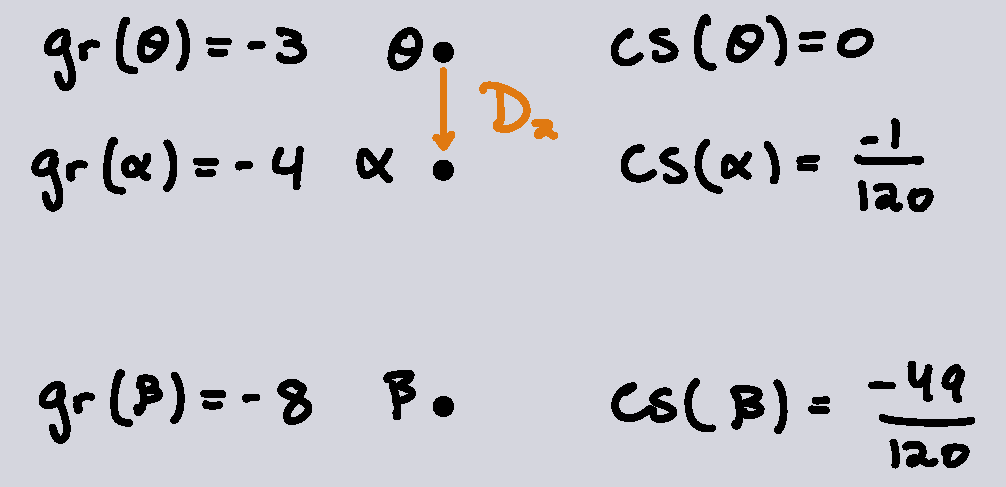
\includegraphics[width=0.55\linewidth]{figures/fig_lec15_example_complex.png}
\end{center}

Is it possible that there is a $\pi_1=1$ self-homology cobordism? If so, it induces a cobordism map. Since $H_1=0$, $\Theta\mapsto\Theta$, and since $F_W$ commutes with $D_2$, $\alpha\mapsto\alpha$. However, sending $\alpha$ to itself is not strictly filtered.
\begin{center}
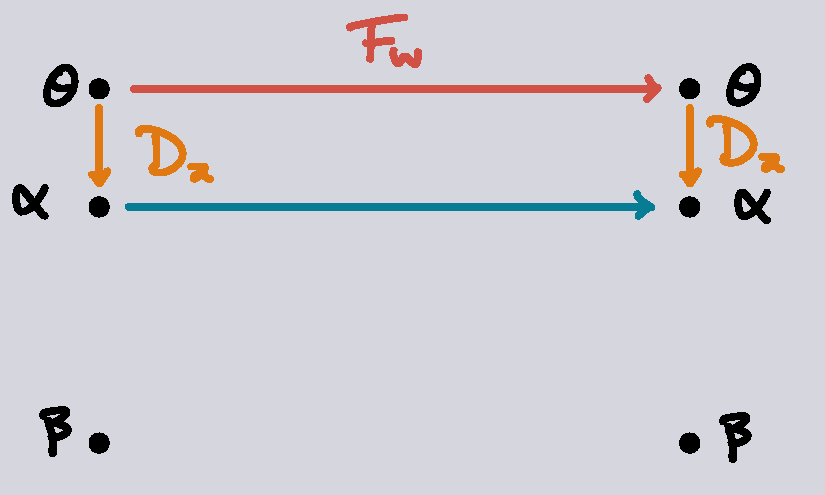
\includegraphics[width=0.4\linewidth]{figures/fig_lec15_no_filtered.png}
\end{center}
Therefore $W$ cannot be simply connected.
\end{example}
\addtocounter{theorem}{-1}\endgroup

However, $-\Sigma(2,3,5)$ does bound a positive-definite manifold. This is consistent with the fact that if we dualized our complex, $[D_2]$ would be $0$:
\begin{center}
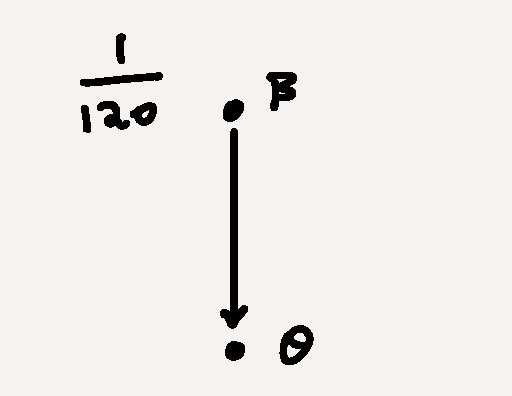
\includegraphics[width=0.25\linewidth]{figures/fig_lec18_dual_complex.png}
\end{center}

The point here is that it's not very easy to use $D_2$ alone to obstruct a $3$-manifold from bounding both types of definite $4$-manifolds. In fact, it's impossible.

\begin{proposition}
With $\mathbb{Q}$-coefficients, at least one of $[D_2^Y]$ and $[D_2^{-Y}]$ is always $0$.
\end{proposition}

This follows from the relation that $D_2\circ D_1\simeq 0$. We've mentioned that the $D_2$ class of $Y$ corresponds to the $D_1$ class of $-Y$, but we haven't actually said what this correspondence actually is. It turns out that there exists a map from the instanton Floer complex to itself, $v:C_\ast\to C_{\ast-4}$ such that
\[
D_2\circ D_1 = 4(\partial v-v\partial),
\]
e.g., $D_2\circ D_1$ is nullhomotopic in $\mathbb{Q}$ coefficients, since $\partial v-v\partial$ is nullhomologous. This brings us to the following:

\begin{proof}[Proof (sketch)]
If $D_1$ and $D_2$ are nontrivial, e.g.:
\begin{itemize}
\item $D_1\alpha\neq 0$ for some cycle $\alpha$
\item $D_2(1)$ is a nonzero homology class
\end{itemize}
then
\begin{align*}
(D_2\circ D_1)(\alpha) &= 4(\partial v-v\partial)(\alpha)\\
&= 4\partial(v\alpha) \quad\text{since $\alpha$ is closed}\\
&\neq 0. \qedhere
\end{align*}
\end{proof}

This is why the second question is interesting. Well, what about $r_s$? Well, it's badly behaved under orientation reversal, so there's hope that it can give the answer, which turns out to be true.

\begin{theorem}[NST]
$2\Sigma(2,3,5)\#-\Sigma(2,3,11)$ does not bound any definite manifold.
\end{theorem}

Recall that $-\Sigma(2,3,6n-1)=S_{1/n}(T_{2,3})$, so
\begin{align*}
-\Sigma(2,3,5) &= S_{+1}(T_{2,3}) =: Y_1,\\
-\Sigma(2,3,11) &= S_{1/2}(T_{2,3}) =: Y_2.
\end{align*}

\begin{proof}
First, we show that $-2Y_1\#Y_2$ does not bound a negative-definite manifold. For this we use the $r_0$-invariant. Last time, we constructed a $\pi_1=1$ cobordism, so $r_0(Y_2)<r_0(Y_1)$. Rewrite $Y_2=Y_1\#Y_1\#(-2Y_1\#Y_2)$. By the $\#$ formula,
\begin{align*}
r_0(Y_2) &= r_0\big(Y_1\#Y_1\#(-2Y_1\#Y_2)\big)\\
&= \min\{r_0(Y_1),\ r_0(-2Y_1\#Y_2)\}.
\end{align*}
Since $r_0(Y_2)<r_0(Y_1)$, we must have that $r_0(-2Y_1\#Y_2)<r_0(Y_1)$, e.g., is finite. Therefore $-2Y_1\#Y_2$ cannot bound a negative-definite $W$.

The intuition is that a negative definite cobordism picks up the minimum.

To show that $-2Y_1\#Y_2$ does not bound a positive-definite manifold, we can equivalently show that $2Y_1\#-Y_2$ does not bound a negative-definite manifold. Consider the unfiltered instanton homology. The essential part of the complex is the flow(s) out of $\Theta$, which for $Y_1$ and $Y_2$ as given are:
\begin{center}
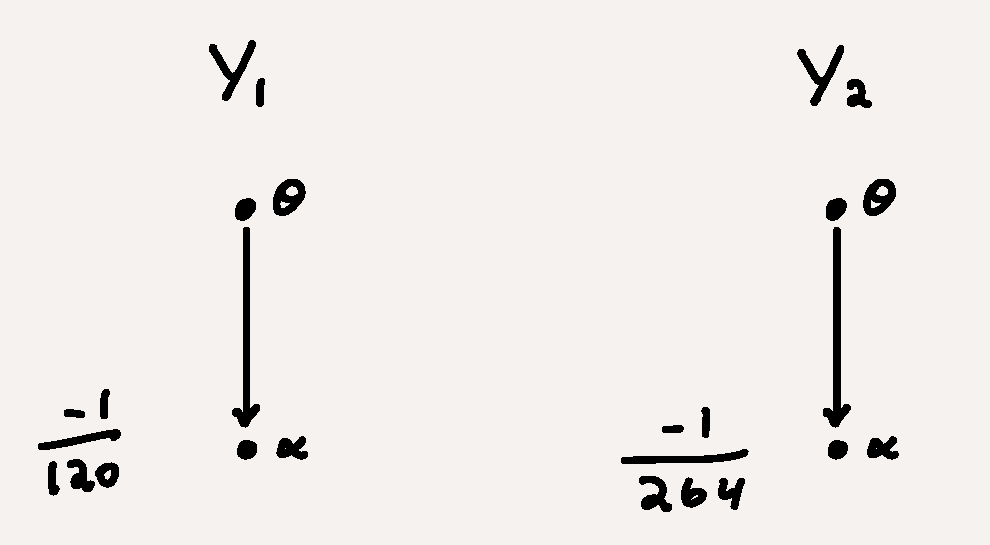
\includegraphics[width=0.5\linewidth]{figures/fig_lec18_complexes.png}
\end{center}
(This is true for the whole family; the only difference is that the filtration level of $\alpha$ gets closer to $0$)
\[
120 = \textcolor{red}{\gcd?}(2\cdot 3,\ 2\cdot 5,\ 3\cdot 5)
\]
In fact, the complex takes this form for the entire family $-\Sigma(2,3,6n-1)$, the only difference being the filtration level of $\alpha$:
\[
\CS(\alpha) = \frac{-1}{24(6n-1)}\cdot(\textcolor{red}{?})
\]
Therefore, from the point of view of unfiltered instantons, these complexes are the same, so $Y_2\sim Y_1$ and $2Y_1\#-Y_2\sim 2Y_1\#-Y_1\sim Y_1$. But $[D_2^{Y_1}]\neq 0$, so $[D_2^{2Y_1\#-Y_2}]\neq 0$. \qedhere
\end{proof}

\begin{remark}
Works like the HF $d$-invariant.
\end{remark}

\subsection*{Linear Independence of Whitehead Doubles}

Recall that if $P$ is a pattern, the operation of satelliting a knot $K$ to $P$ is a map from the smooth concordance group to itself: $P$ induces a map $P:\mathcal{C}^{\mathrm{SM}}\to\mathcal{C}^{\mathrm{SM}}$.

What's interesting about this map is that it's not usually a homomorphism. It's an old and deep question: for different $P$'s, what is the nature of this map? One particularly interesting $P$ is the Whitehead doubling pattern:
\[
\mathrm{Wh} : \mathcal{C}\to\mathcal{C}
\]
\begin{center}
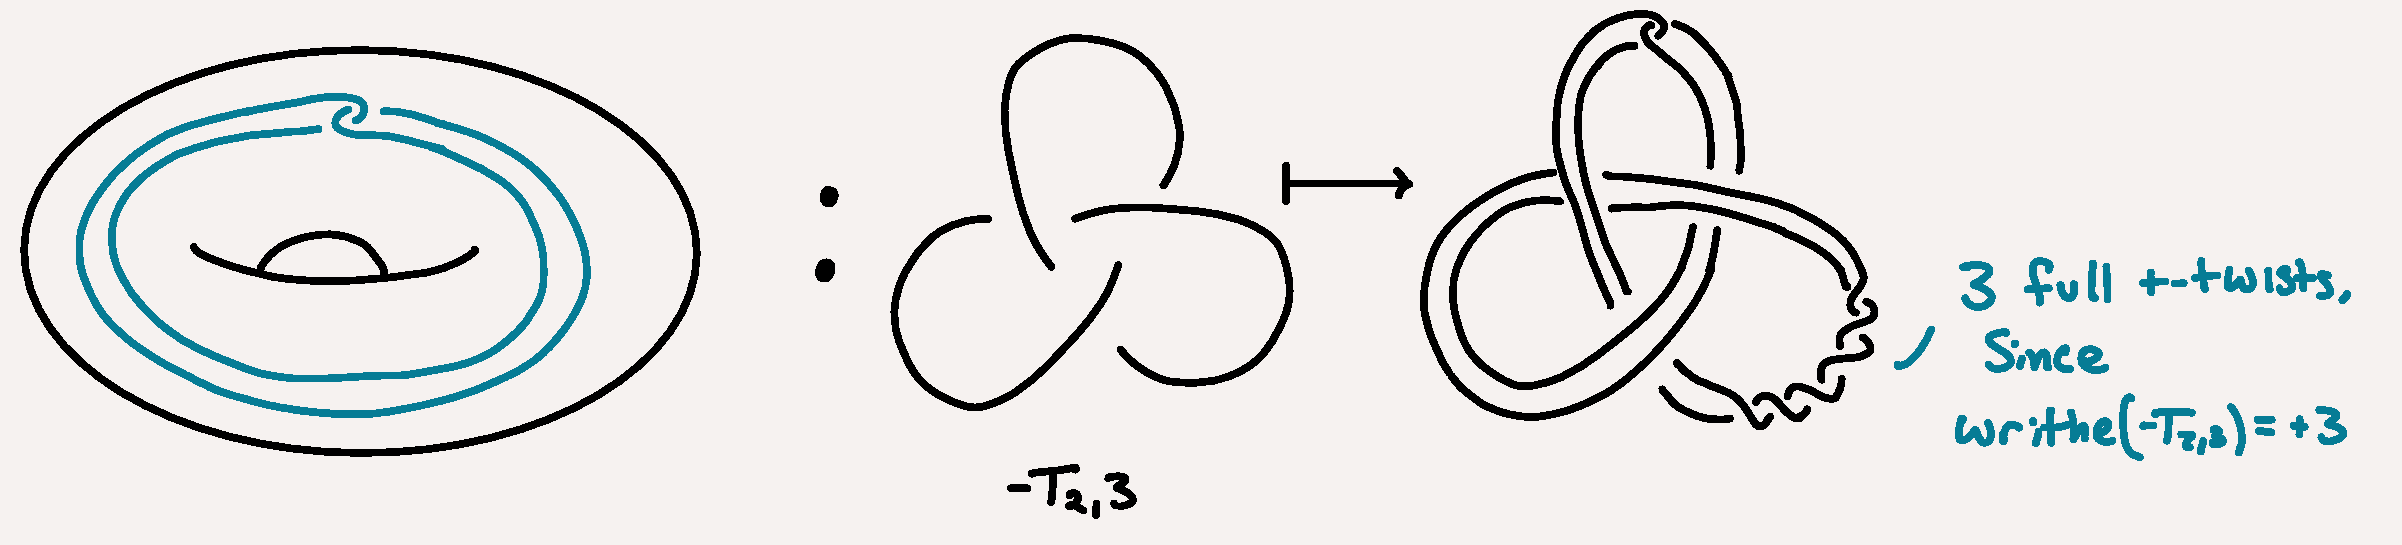
\includegraphics[width=0.9\linewidth]{figures/fig_lec18_wh_pattern.png}
\end{center}

\begin{question}
Is $\mathrm{Wh}$ (weakly) injective?
\end{question}
This question is still open and is considered very difficult. To resolve it, one must find some $K$ for which $\mathrm{Wh}(K)$ is smoothly slice, but $K$ isn't, or prove no such $K$ exists. For example, it's unknown if $\mathrm{Wh}(-T_{2,3})$ is slice (though $-T_{2,3}$ isn't).

\begin{question}
Is $\mathrm{Wh}$ injective?
\end{question}
Since $\mathrm{Wh}$ is not a homomorphism, the question of weak injectivity is distinct from that of usual injectivity: does there exist knots $K_1,K_2$ such that $\mathrm{Wh}(K_1)$ is concordant to $\mathrm{Wh}(K_2)$ but $K_1$ is not concordant to $K_2$. This is also still open, as well as the following.

\begin{question}
Does $\mathrm{Wh}$ preserve linear independence?
\end{question}
This was a conjecture of Hedden and Kirk from the 90's, though the question has existed for much longer. Their conjectured answer was yes. At the time it was posed, it was very hard to attack it. In fact, in their paper, they didn't even produce an example of a pair of linearly independent knots whose Whitehead doubles are also linearly independent. One amusing fact is that there are knots $K$ for which $\{\mathrm{Wh}(nK)\}_{n=1}^\infty$ are linearly independent, so $\mathrm{Wh}$ is really not a homomorphism. It spreads out the span of what it feeds in.

It is still very hard to attack this problem for two main reasons:
\begin{enumerate}
\item $\mathrm{Wh}(K)$ is topologically slice, so no classical algebraic invariant will work. Thus we need an invariant distinguishing topological and smooth sliceness.
\item $\mathrm{Wh}(K)$ has Seifert genus $1$. This means that HFK of $\mathrm{Wh}(K)$ is small, e.g., it vanishes outside a grading range which depends on the Seifert genus. Therefore, obtaining a linear independence result for an $\infty$ set is very difficult, since there's not enough room in HFK to obstruct concordance. However, note that in his thesis, Hedden did do it for a finite set for specific $K$'s.
\end{enumerate}

The point here is that it's hard to use existing invariants to establish linear independence of an $\infty$-family. So what can we do? Let's translate this question into a question about $3$-manifolds, and ask about homology cobordism instead. Recall the definition of a double branched cover.

\begin{definition}
A map $f:X^n\to Y^n$ is a branched covering if there exists $B^{n-2}\subseteq Y$ such that $f:X\setminus f^{-1}(B)\to Y\setminus B$ is a covering map and $f$ is $1:1$ on the branch locus.

$B:=$ branch set, $f^{-1}(B):=$ branch locus.
\end{definition}

\begin{definition}
The double branched cover of a knot $K\subset S^3$ is a $3$-manifold $\Sigma_2(K)$ and covering map $f:\Sigma_2(K)\to S^3$ such that $f_\ast:\pi_1(\Sigma_2(K)\setminus f^{-1}(K))\to\pi_1(S^3\setminus K)$ is injective, with image the kernel of the homomorphism $\pi_1(S^3\setminus K)\to\mathbb{Z}/2$ sending a meridian $\mu$ to $1$.
\end{definition}

\[
\Sigma_2 : \mathcal{C}\longrightarrow\Theta^3_{\mathbb{Z}/2}, \qquad K\longmapsto\Sigma_2(K)
\]

It turns out that this is a well-defined homomorphism to $\Theta^3_{\mathbb{Z}/2}$.

The point here is that taking the branched cover of a concordance gives a cobordism, so obstructing such a cobordism obstructs concordance. We have methods for this via the $r_0/r_s$ invariant with $\mathbb{Z}/2$ coefficients!

\begin{remark}
We have been (somewhat sloppily) ignoring signs anyway, so using $\mathbb{Z}/2$ instead of $\mathbb{Z}$ shouldn't be too much of a change.
\end{remark}

Using $\Sigma_2$ is especially convenient for Whitehead doubles since
\[
\Sigma_2(\mathrm{Wh}(K)) = S_{\frac{1}{2}}(K\#K):
\]
Given $K\subset S^3$, first take $K\#K^{(r)}$.
\begin{center}
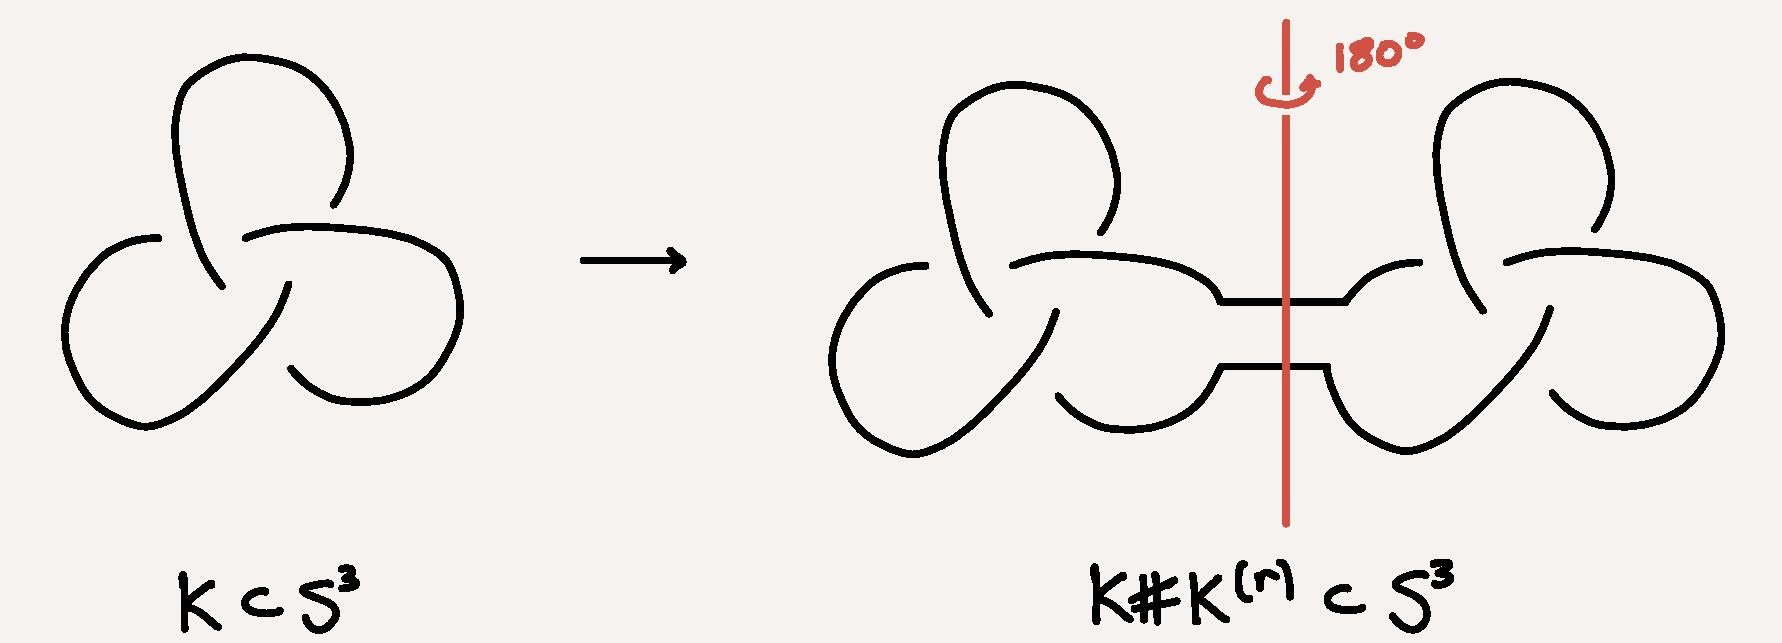
\includegraphics[width=0.9\linewidth]{figures/fig_lec18_k_kr.png}
\end{center}
Note that there is a symmetry of $S^3$ which fixes $K\#K^{(r)}$ setwise given by $180^\circ$ rotation about the shown axis. Now, take a tubular neighborhood of $K\#K^{(r)}$ and quotient by this rotation.
\begin{center}
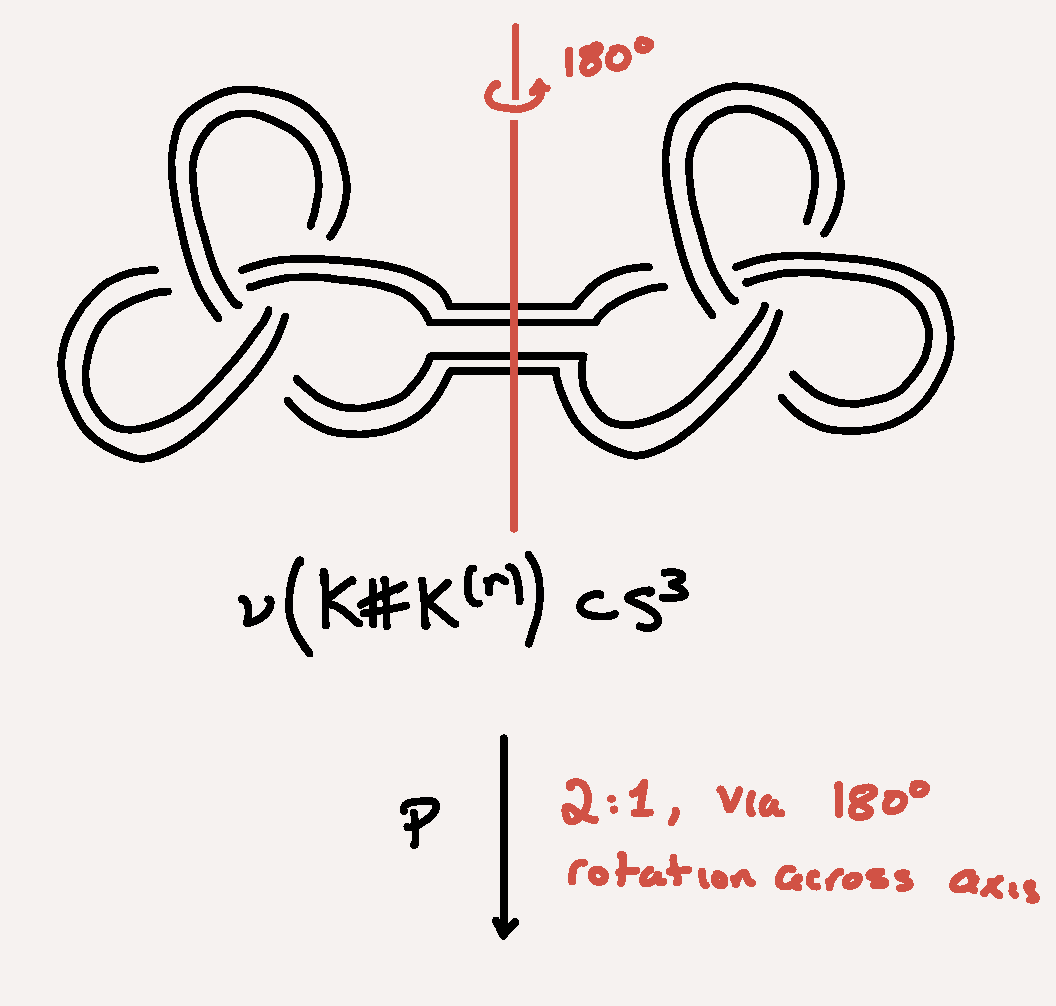
\includegraphics[width=0.4\linewidth]{figures/fig_lec18_nbhd_rotation.png}
\end{center}
\begin{center}
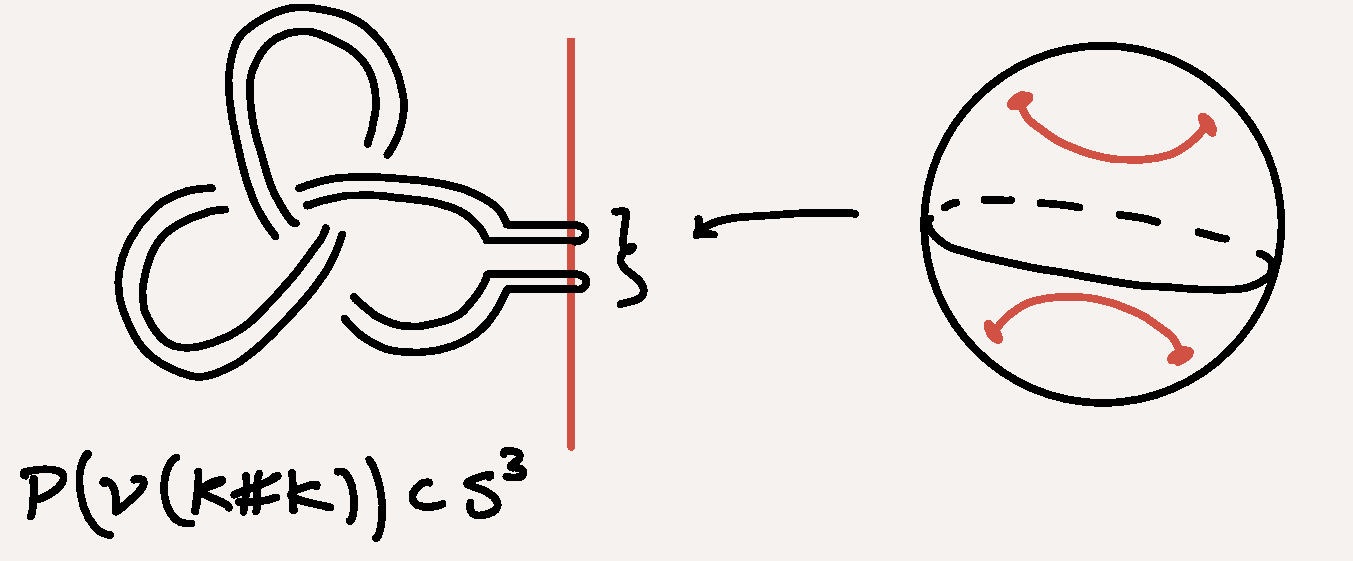
\includegraphics[width=0.75\linewidth]{figures/fig_lec18_quotient_ball.png}
\end{center}

$P(\nu(K\#K))$ is a ball which intersects the branch locus in two boundary-parallel arcs. Before the quotient, surgery on $K\#K$ corresponded to removing $\nu(K\#K)$ and regluing by some map from the boundary torus to itself. However, in this branch locus, surgery corresponds to ripping out this ball and regluing it by some twist, or, equivalently, a different tangle. Since this ball contains the branch locus, this surgery changes the locus, which changes the branch set upstairs. This is called ``rational tangle replacement'', where the surgery coefficient $p/q$ determines the tangle, and vice versa. For the Whitehead double, the corresponding tangle replacement is
\begin{center}
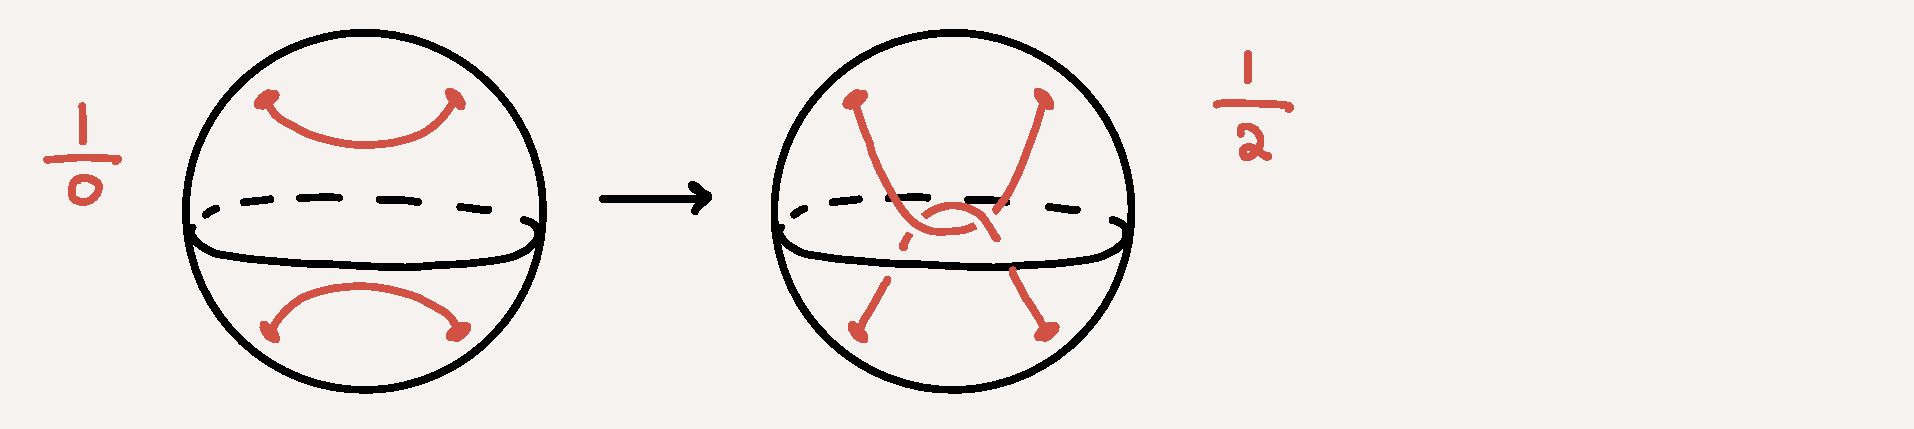
\includegraphics[width=0.75\linewidth]{figures/fig_lec18_tangle_replacement.png}
\end{center}
and the branch locus becomes
\begin{center}
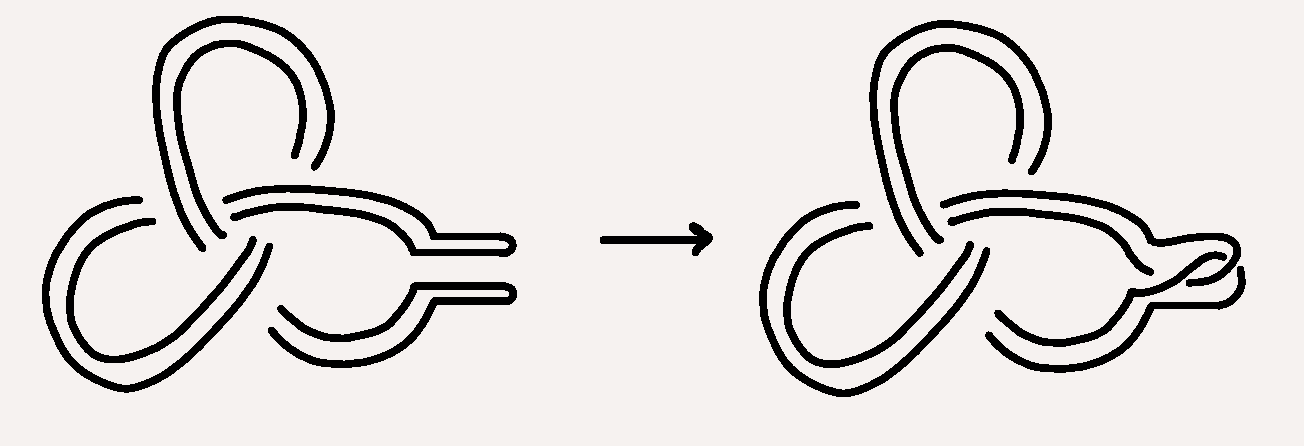
\includegraphics[width=0.6\linewidth]{figures/fig_lec18_branch_locus.png}
\end{center}

Note that $S_{1/2}(K\#K)$ is a $\mathbb{Z}\mathrm{HS}^3$. Now we've turned a question about linear independence into a question about distinguishing $\mathbb{Z}\mathrm{HS}^3$'s in $\Theta^3_{\mathbb{Z}/2}$, which is the sort of question we know how to answer. We should be able to calculate some of the IFH invariants coming from manifolds like $S_{1/2}(K\#K)$.

In light of the full conjecture, this theorem is not super impressive, but it is the first major progress on it.

\begin{theorem}[NST]
$\mathrm{Wh}(T_{2,2n+1})$ are linearly independent.
\end{theorem}

There are other families to which this argument can be applied, but we'll outline the proof for the $T_{2,2n+1}$ torus knots for simplicity.

\begin{proof}
Define $Y_n := S_{1/2}(T_{2,2n+1}\#T_{2,2n+1})$. Then $Y_n=\Sigma_2(\mathrm{Wh}(T_{2,2n+1}))$.

It suffices to show that the $\{Y_n\}_{n\geq 1}^\infty$ are linearly independent in $\Theta^3_{\mathbb{Z}/2}$. We'll use the general algebraic theorem from last time, so we need to know:
\begin{itemize}
\item[2)] $\infty=r_0(-Y_1)=r_0(-Y_2)=\dots$

This is true since $Y_n$ is $-\frac{1}{2}$ surgery on $K$.
\item[1)] $\infty>r_0(Y_1)>r_0(Y_2)>\dots$

We'll similarly construct a negative-definite cobordism from $Y_n$ to $Y_{n+1}$
\end{itemize}
\begin{center}
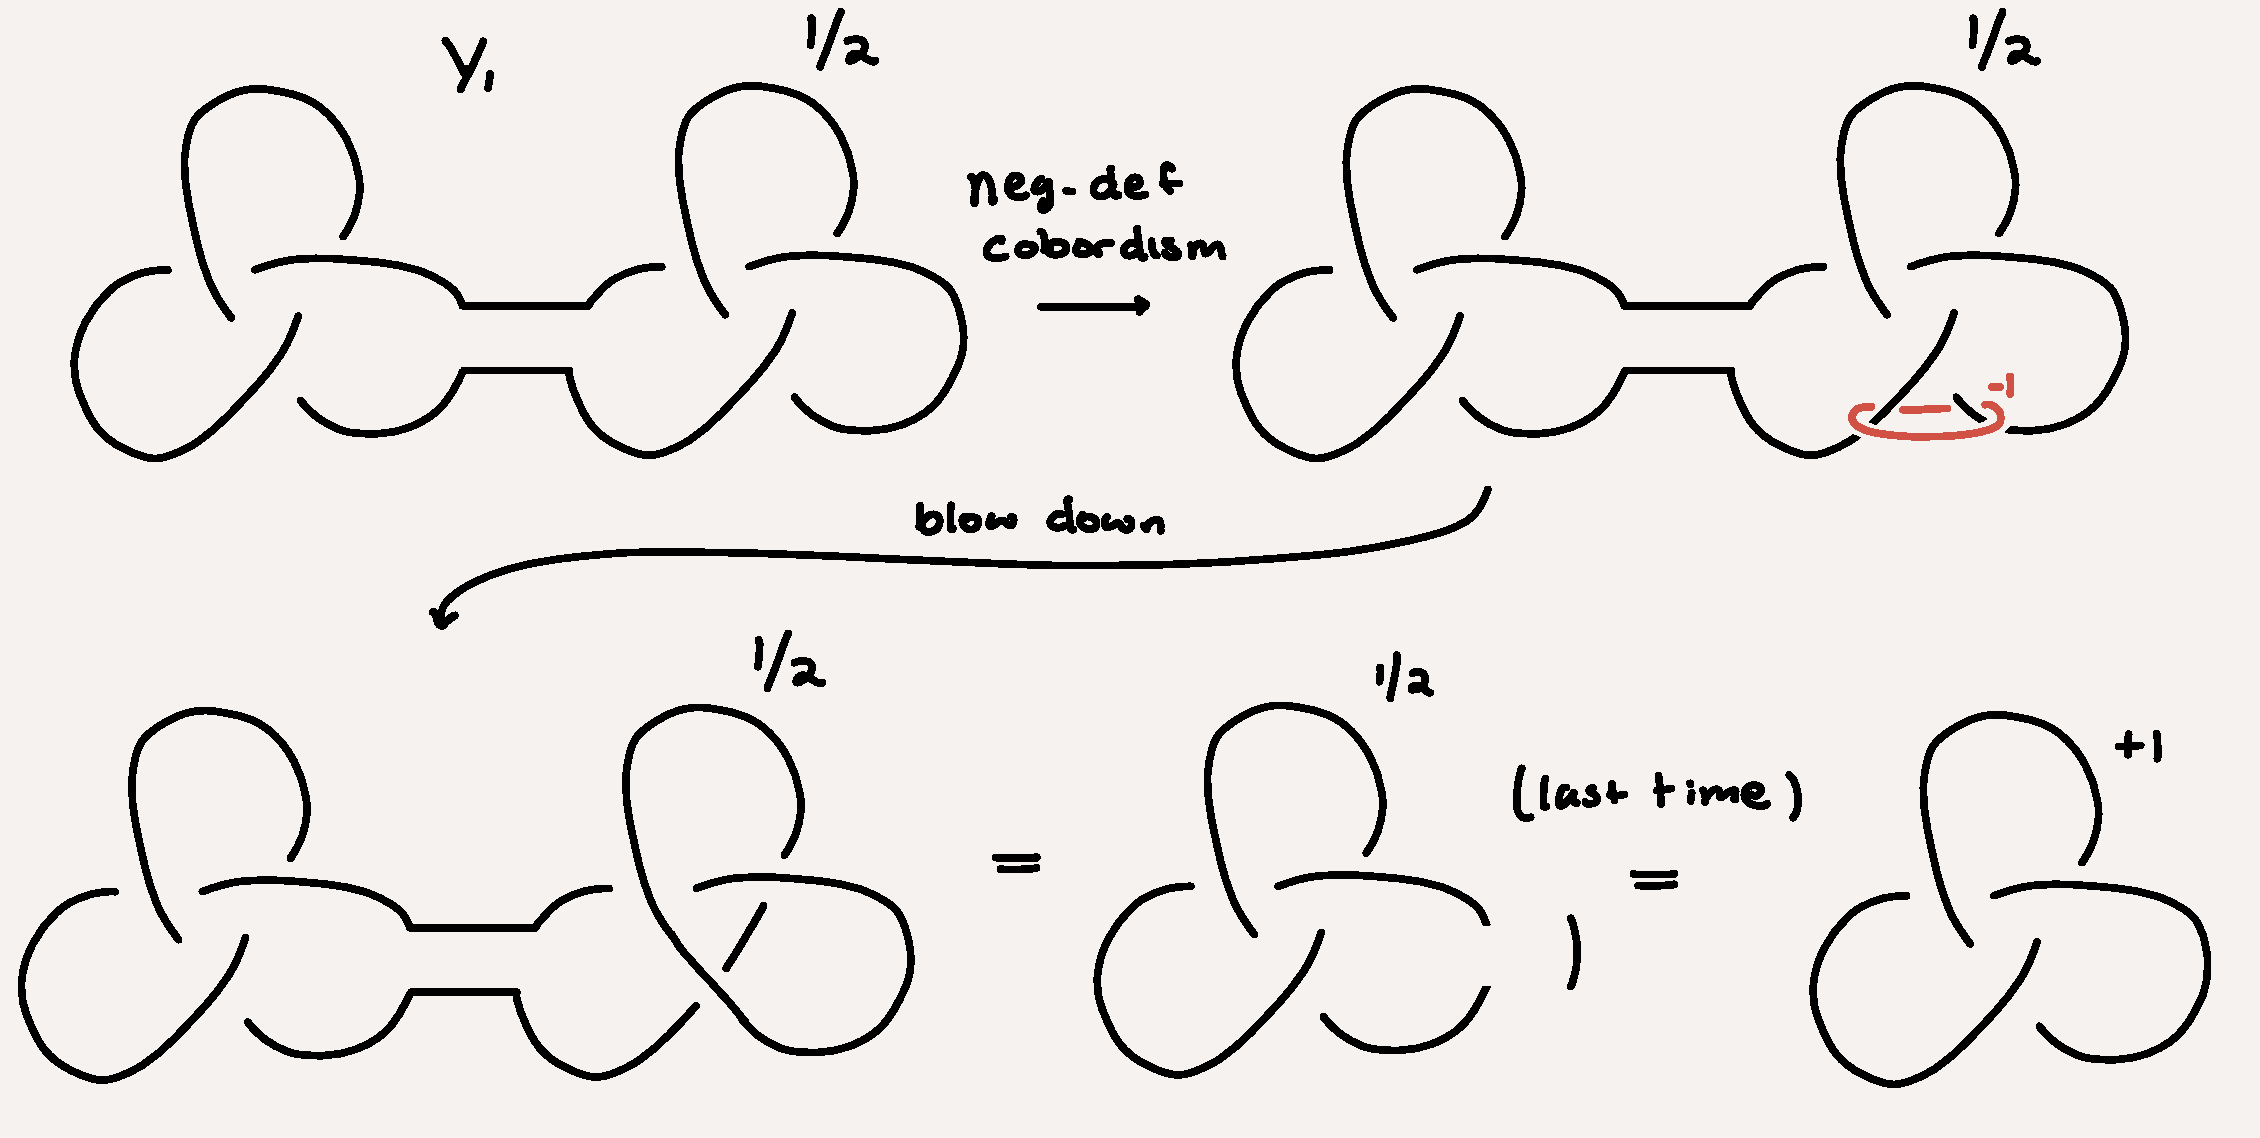
\includegraphics[width=0.95\linewidth]{figures/fig_lec18_negdef_cob.png}
\end{center}
More generally, the picture is
\begin{center}
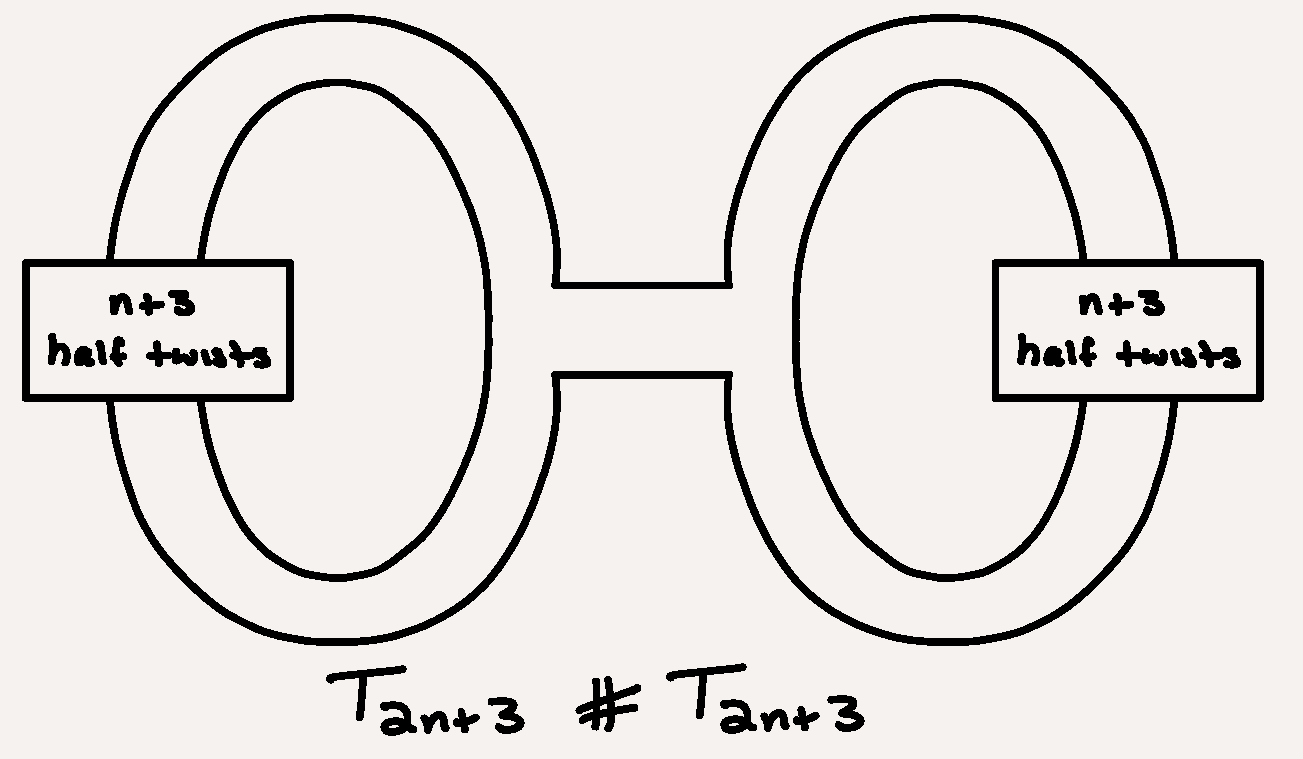
\includegraphics[width=0.5\linewidth]{figures/fig_lec18_general_picture.png}
\end{center}
where the cobordism handle attachment and subsequent blowdown decrease the number of half twists on each side by $2$:
\begin{center}
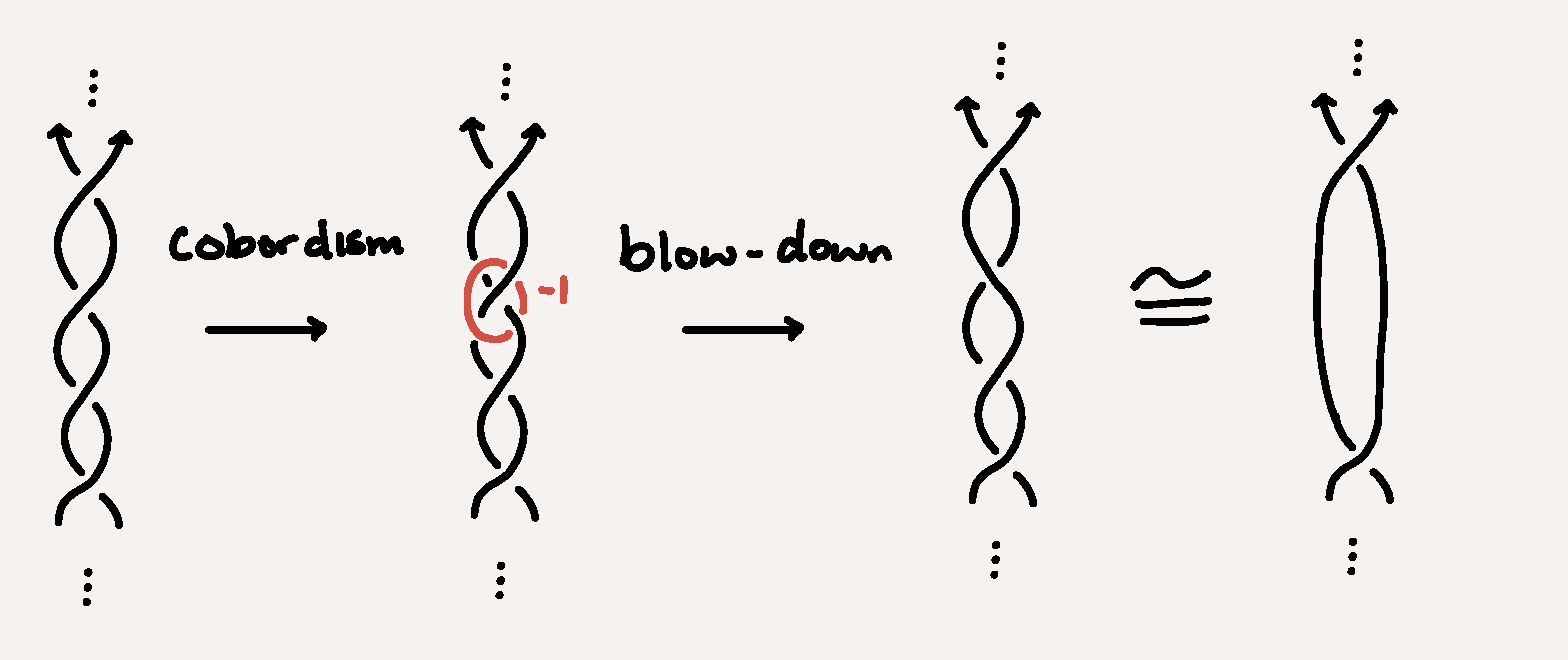
\includegraphics[width=0.75\linewidth]{figures/fig_lec18_twist_reduction.png}
\end{center}
This gives a negative-definite cobordism from $T_{2n+3}\#T_{2n+3}$ to $T_{2n+1}\#T_{2n+1}$. \qedhere
\end{proof}

To finish our discussion of the NST paper, we'll address some open questions they mention.

\subsection*{Rationality of CS}

\begin{question}
Are the critical values of the CS functional always rational?
\end{question}

You may have noticed that, at least in our examples, $\CS(\rho)=\frac{1}{\#}$. The issue is that the only things we've computed CS for are Brieskorn spheres and graph manifolds, all of which have rational CS values. However, the answer to this question is probably no.

In the NST paper they propose a counterexample -- there are actually many different counterexamples, some of which we expect aren't rational. The primary two are $S^3_{1/2}(-5_2)$ and $S^3_{1/2}(4_1)$.

The CS functionals can be numerically approximated, and they don't look rational, but this isn't an obstructive proof.

For $-5_2$, $r_0$ is believed to be non-rational, and they present consequences of this, if true.

Suppose you have a class of $3$-manifolds all of which have rational CS values. In the tensor product complex for $\#$, these must have rational CS, so the $r_s$ invariant is rational, so there cannot be any $3$-manifold in this span with irrational CS value.

A few months ago, Nozaki showed that $-5_2$ is not in the span of graph manifolds, which negatively answered the open question of whether the span of all graph manifolds is $\Theta^3_{\mathbb{Z}}$.

\end{document}
